\chapter{MOC Parameter Sensitivity Studies}
\label{chap:moc-sensitivity}

In this chapter, sensitivity to both mesh refinement and \ac{MOC} ray refinement is studied in detail. First, radial sensitivity is analyzed in Section~\ref{sec:radial-sensitivity} and in Section~\ref{sec:axial-sensitivity} axial sensitivity is studied. Both sections conduct both mesh refinement and ray refinement studies assuming a linear source approximation. In Section~\ref{sec:flat-linear-comparison}, a comparison of flat and linear source solvers is presented.

%%%%%%%%%%%%%%%%%%%%%%%%%%%%%%%%%%%%%%%%%%%%%%%%%%%%%%%%%%%%%%%%%%%%%%%%%%%%%%%%
\section{Radial Sensitivity}
\label{sec:radial-sensitivity}

Due to long experience with 2D \ac{MOC}, the radial parameters required to achieve sufficient accuracy -- both in mesh and ray refinement -- are relatively well known. These requirements for linear source were thoroughly studied by Ferrer~\cite{ferrer2012linear}. Based on these studies and CASMO-5 default parameters~\cite{rhodes2006casmo}, the expected radial parameters needed to achieve a sufficiently accurate solution are given in Table~\ref{tab:expected-radial-params}. Each of the parameters listed in the table will be thoroughly discussed and undergo a refinement study.

\begin{table}[ht]
	\centering
	\caption{Expected radial MOC parameters to sufficiently resolve the \ac{MOC} fission distribution using a linear source approximation}
	\medskip
	\begin{tabular}{lc}
		\hline
		Number of Rings in Fuel and Moderator & 1 \\
		Number of Sectors in Fuel & 4 \\
		Number of Sectors in Moderator & 8 \\
		Number of Sectors in Guide Tubes & 8 \\	
		Radial Ray Spacing & 0.05 cm \\
		Number of Azimuthal Angles & 64 \\
		Reflector Mesh & $3 \times 3$ cells per pin-cell mesh \\
		\hline
	\end{tabular}
	\label{tab:expected-radial-params}
\end{table}

\subsection{Core Radial Mesh Refinement}

First, the radial mesh within the core is studied. The core is composed of a lattice of assemblies. Therefore, the mesh refinement can be studied on a single assembly model. Since the axial dimensions should not largely impact the radial sensitivity the BLANK model is used, which is a 10 cm tall single assembly region without any grid spacers and reflective boundary conditions placed in both axial directions. This problem is simulated with the \ac{MOC} ray parameters given in Table~\ref{tab:rad-mesh-refinement-params}. These parameters are quite fine in the radial direction in order to accurately test the impact of the radial mesh. In the axial direction, the source height and axial ray spacing are quite coarse as the problem is uniform axially with no physical axial flux shape.

\begin{table}[ht]
	\centering
	\caption{XXX}
	\medskip
	\begin{tabular}{lc}
		\hline
		Radial Ray Spacing & 0.025 cm \\
		Number of Azimuthal Angles & 128 \\
		Axial Ray Spacing & 3.0 cm \\
		Number of Polar Angles & 10 \\
		Axial Source Height & 10.0 cm \\
		\hline
	\end{tabular}
	\label{tab:rad-mesh-refinement-params}
\end{table}

Typically, pin-cells are discretized into rings and sectors, as presented in Figure~\ref{fig:rings-sectors}. Ring divisions help to capture radial variation within the pin-cell and sector divisions help to capture angular variation.

\begin{figure}[h!]
	\centering
	\begin{subfigure}{0.3\textwidth}
		\centering
		
\includegraphics[width=\linewidth]{figures/simp_fuel_pin.png}
		\caption{}
		\label{fig:rings-sectors-a}
	\end{subfigure}
	\begin{subfigure}{0.3\textwidth}
		\centering
		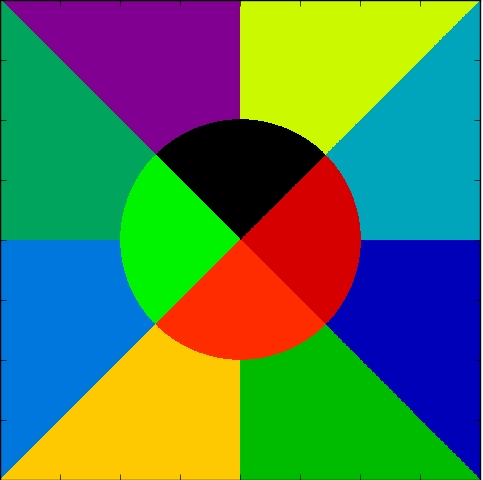
\includegraphics[width=\linewidth]{figures/sector_discr.jpg}
		\caption{}
		\label{fig:rings-sectors-b}
	\end{subfigure}
	\begin{subfigure}{0.3\textwidth}
		\centering
		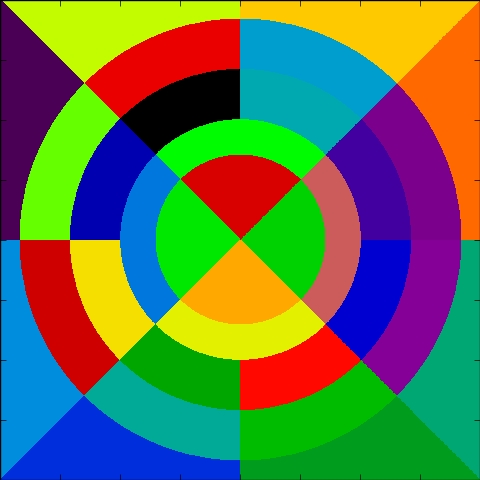
\includegraphics[width=\linewidth]{figures/ring_sector_discr.jpg}
		\caption{}
		\label{fig:rings-sectors-c}
	\end{subfigure}
	\caption[]{A simplified pin-cell (a) of just moderator and homogenized fuel is discretized (b) into 8 sectors in the moderator and 4 sectors in the fuel and further discretized (c) into 2 rings in the fuel and 3 rings in the moderator.}
	\label{fig:rings-sectors}
\end{figure}

While the illustration in Figure~\ref{fig:rings-sectors} only shows fuel and moderator regions, realistic pin-cells contain fuel, gap, clad, and moderator. For mesh refinement, ring divisions are never added in gap and clad regions since they are so thin. However, sector divisions are added in these regions. In our studies, the sector divisions within fuel is also applied to the associated gap and clad regions.

Since both fuel pins and guide tubes exist in fuel assemblies, there are three main zones of interest that could be independently discretized: fuel pins, guide tubes, and moderator.

\subsubsection{Ring Divisions}

First, ring divisions are studied. The number of rings is counted by the number of \texttt{ZCylinder} surfaces bounding the region. For instance, 1 ring implies no further discretization in the regions. 

For fuel rods and guide tubes, these rings divide the regions by creating concentric \texttt{ZCylinder} surfaces inside the rod such that the volume of all regions are equal. For moderator regions, \texttt{ZCylinder} objects are created outside the rod in concentric circles such that the distance between the surfaces is equal. Since there is no bounding outer \texttt{ZCylinder}, a virtual bounding \texttt{ZCylinder} is created with volume equal to that of the pin-cell.

The sensitivity studies of ring divisions are shown in Table~\ref{tab:ring-sensitivity}. For all cases, the expected radial mesh parameters are used unless otherwise specified. For each zone, a separate parameter refinement is conducted using 1, 2, and 3 rings. The 3 ring case is always chosen as the reference. For the other radial mesh parameters, expected parameters are used (1 ring in all regions with 4 sectors in fuel and 8 sectors in the moderator and guide tube).

\begin{table}[ht]
	\centering
	\caption{MOC sensitivity to mesh refinement by radial rings in fuel, guide tube, and moderator regions}
	\medskip
	\begin{tabular}{c|c|c|c|c|c|c}
		\hline
		 & No. of & Ref. & & $k_{\textit{eff}}$ & RMS Fission & Max Fission \\
		Region & Rings  & Rings & $k_{\textit{eff}}$ & Bias & Rate Error & Rate Error \\
		\hline
		Fuel & 1 & 3 & 1.21568 & 0.9 pcm  & 0.002 \% & 0.003 \% \\
		Fuel & 2 & 3 & 1.21569 & 0.4 pcm  & 0.001 \% & 0.002 \% \\
		Fuel & 3 & 3 & 1.21569 & -- & -- & -- \\
		\hline
		\hline
		Guide Tube & 1 & 3 & 1.21569 & 0.1 pcm & 0.002 \% & 0.004 \% \\
		Guide Tube & 2 & 3 & 1.21569 & <0.1 pcm  & 0.002 \% & 0.004 \% \\
		Guide Tube & 3 & 3 & 1.21569 & <0.1 pcm & -- & -- \\
		\hline
		\hline
		Moderator & 1 & 3 & 1.21569 & 4.7 cm  & 0.003 \% & 0.007 \% \\
		Moderator & 2 & 3 & 1.21564 & -0.3 pcm  & 0.002 \% & -0.004 \% \\
		Moderator & 3 & 3 & 1.21564 & -- & -- & -- \\
		\hline
	\end{tabular}
	\label{tab:ring-sensitivity}
\end{table}

These results show very little sensitivity. With a linear source approximation, gradients can be accurately captured without further radial discretization, causing ring divisions to be less important. The most sensitivity is observed in the moderator region, but still less than 5 pcm. Therefore, all tests in this study do not use ring discretizations. 

\subsubsection{Sector Divisions}

Next, radial discretization into sectors in analyzed. Since these  discretizations largely account for angular differences rather than spatial gradients, they might still be needed with a linear source approximation. Again, the three regions (fuel, guide tubes, and moderator) are analyzed separately. Recall that gap and clad are discretized into the same number of sectors as the rod they surround.

For all of the cases, the RMS and maximum fission rate error is inconsequential, similar to that observed with discretization by rings.  The maximum error occurred when comparing a case without any sector discretization for moderator, in which the RMS fission rate error was 0.1\% and the maximum fission rate error was 0.3\%, which are both fairly low. However, the effect on the eigenvalue $k_{\textit{eff}}$ was more substantial. Therefore, the results for sector discretization focus on the impact on eigenvalue.

Similar to the approach taken for discretizing by rings, all mesh parameters are taken to be the expected parameters except the parameter being tested. All error estimates are formed relative to 16 sectors. Figure~\ref{fig:fuel-sectors} shows the sensitivity to the sector discretization of fuel and Figures~\ref{fig:gt-sectors} and \ref{fig:mod-sectors} show the same for guide tubes and moderator, respectively.
 
\begin{figure}[h!]
	\centering
	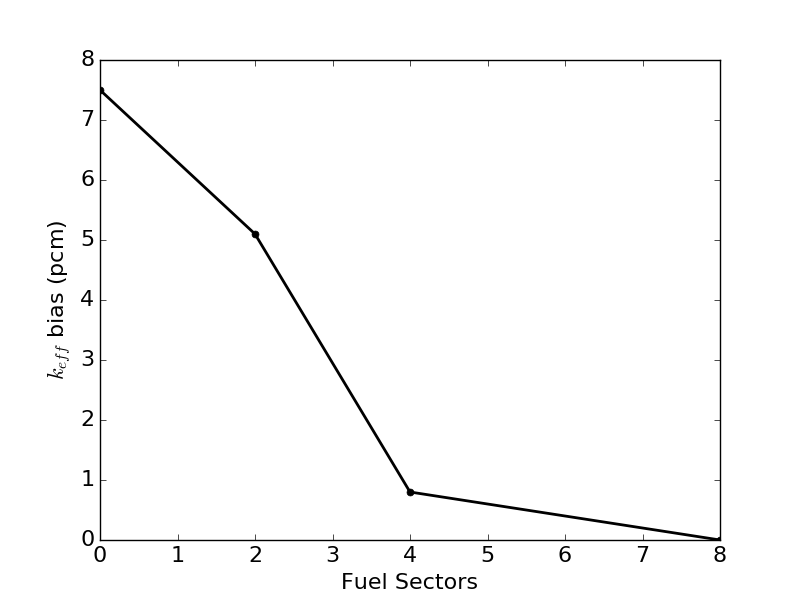
\includegraphics[width=0.7\linewidth]{figures/results/sensitivity/fuel_sectors.png}
	\caption[]{The bias in eigenvalue $k_{\textit{eff}}$ decreasing as the number of sector discretizations increased in fuel rod.}
	\label{fig:fuel-sectors}
\end{figure}
\begin{figure}[h!]
	\centering
	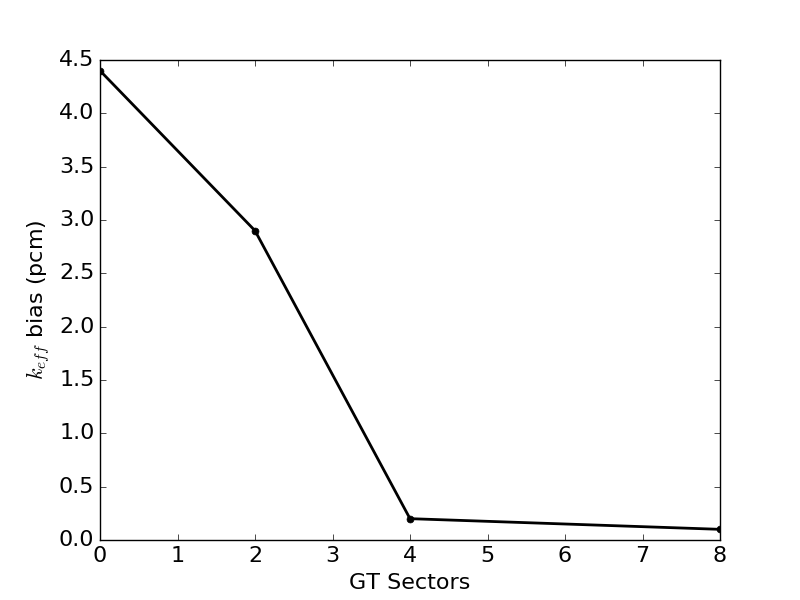
\includegraphics[width=0.7\linewidth]{figures/results/sensitivity/gt_sectors.png}
	\caption[]{The bias in eigenvalue $k_{\textit{eff}}$ decreasing as the number of sector discretizations increased in guid tubes.}
	\label{fig:gt-sectors}
\end{figure}
\begin{figure}[h!]
	\centering
	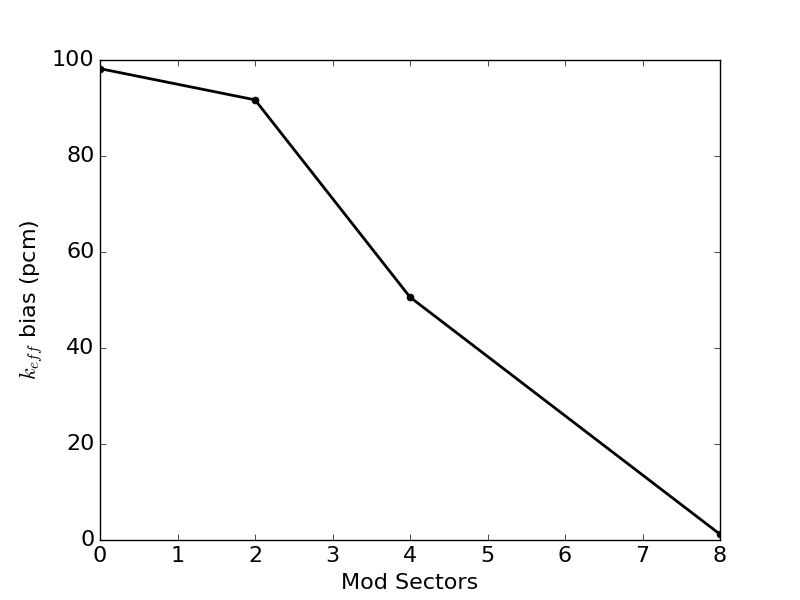
\includegraphics[width=0.7\linewidth]{figures/results/sensitivity/mod_sectors.png}
	\caption[]{The bias in eigenvalue $k_{\textit{eff}}$ decreasing as the number of sector discretizations increased in moderator regions.}
	\label{fig:mod-sectors}
\end{figure}

These results show that the moderator region is again the most sensitive. After 8 sectors in the moderator and 4 in fuel and guide tubes, very little sensitivity is observed. This would imply that requiring 8 sectors in the guide tubes may be excessive, but guide tubes are relatively sparse throughout the core so the increased discretization should not heavily impact computational requirements. Therefore, in order to be conservative, 8 sectors remains the choice for guide tube discretization.

\subsection{Reflector Radial Mesh Refinement}

Ring and sector discretizations form a well-defined mesh refinement within the core. However, for full core problems, the radial water reflector also needs to be discretized. To simplify the sensitivity study, a uniform global mesh is overlaid across the reflector regions. In addition, the discretization is chosen to align with \ac{CMFD} cell boundaries. In OpenMOC, \ac{CMFD} cell boundaries naturally create mesh discretizations as cells are split at the mesh boundaries. Since a pin-cell width uniform \ac{CMFD} mesh is chosen for acceleration of BEAVRS problems, the reflector is naturally discretized into pin-cell-sized regions. The radial mesh refinement then takes the form of a uniform mesh discretization within a pin-cell-sized region. Furthermore, a square mesh refinement is chosen. Since each assembly contains a lattice of $17\times 17$ cells and an assembly width is $\approx 21.5$ cm (when including inter-assembly gap), the radial reflector mesh refinement takes the form of an $N \times N$ discretization of each 1.264 cm $\times$ 1.264 cm region within the reflector.

In order to conduct radial reflector mesh refinement sensitivity studies, a full core model is necessary. However, the full 3D BEAVRS model is computationally demanding. Therefore, the 2D BEAVRS model described in Section~\ref{sec:beavrs-2D} is chosen. This model represents a radial cut of the full core BEAVRS geometry that has been extruded 10 cm in height with reflective boundary conditions placed on the top and bottom of the geometry. With the height greatly reduced from the full 3D model, the computational requirements are far less. In addition, since this model contains no axial variation, the radial sensitivity can be tested more directly. The \ac{MOC} parameters used in this sensitivity study are presented in Table~\ref{tab:rad-ref-refinement-params}.


\begin{table}[ht]
	\centering
	\caption{XXX}
	\medskip
	\begin{tabular}{lc}
		\hline
		Radial Ray Spacing & 0.1 cm \\
		Number of Azimuthal Angles & 32 \\
		Axial Ray Spacing & 1.5 cm \\
		Number of Polar Angles & 10 \\
		Axial Source Height & 2.0 cm \\
		\hline
	\end{tabular}
	\label{tab:rad-ref-refinement-params}
\end{table}

The results of the sensitivity study are presented in Figures~\ref{fig:rad-ref-pcm} and ~\ref{fig:rad-ref-fr} for eigenvalue and fission rate, respectively. All sensitivities are compared to a reference solution which uses a $5\times 5$ radial reflector mesh discretization. The results show little sensitivity to the reflector mesh, likely since the linear source approximation is able to accurately capture gradients. At the expected $3 \times 3$ reflector mesh refinement, the eigenvalue bias is below 1 pcm and all relative fission rate biases are below 0.1\%. Therefore, the  $3 \times 3$ radial reflector mesh discretization is sufficient to accurately resolve the solution and is chosen for all further studies and results.

\begin{figure}[h!]
	\centering
	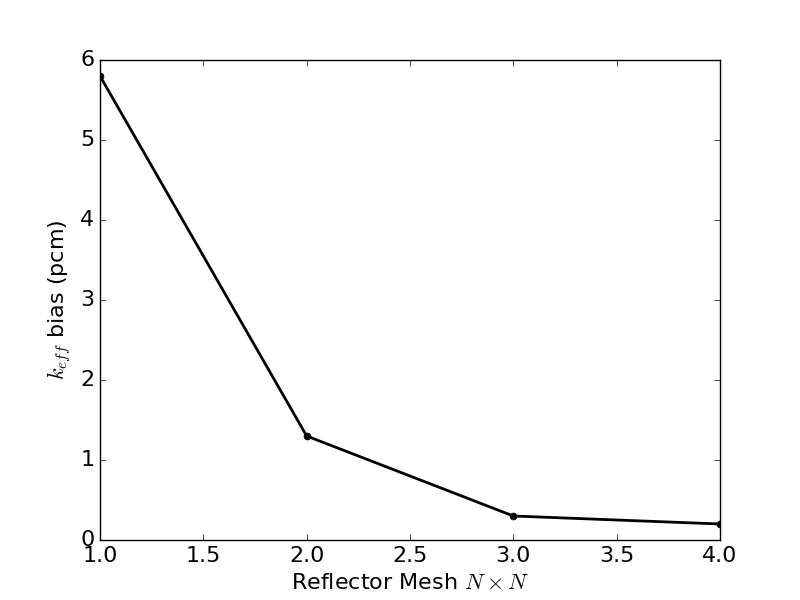
\includegraphics[width=0.7\linewidth]{figures/results/sensitivity/reflector_mesh_pcm.png}
	\caption[]{The bias in eigenvalue $k_{\textit{eff}}$ decreasing as reflector mesh of square discretization $N \times N$, where $N$ is the number of mesh discretizations in each pin-cell width, is refined within the radial water reflector.}
	\label{fig:rad-ref-pcm}
\end{figure}
\begin{figure}[h!]
	\centering
	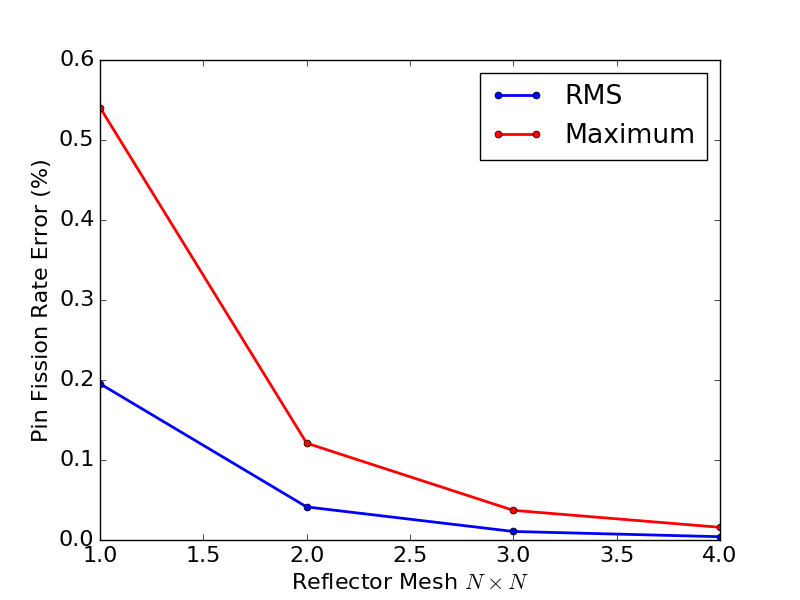
\includegraphics[width=0.7\linewidth]{figures/results/sensitivity/reflector_mesh_fr.png}
	\caption[]{The relative pellet-wise fission rate error decreasing as reflector mesh of square discretization $N \times N$, where $N$ is the number of mesh discretizations in each pin-cell width, is refined within the radial water reflector.}
	\label{fig:rad-ref-fr}
\end{figure}

\subsection{Radial Ray Refinement}

%FIXME
FIXME: discussion

\subsubsection{Radial Ray Spacing Sensitivity}'

%FIXME
FIXME: discussion
ref: 0.0125
base: 32 az angles

[  NORMAL ]  Azimuthal ray spacing = 0.100000
[  NORMAL ]  Number of polar angles = 10
[  NORMAL ]  Z-spacing = 0.750000


\begin{figure}[h!]
	\centering
	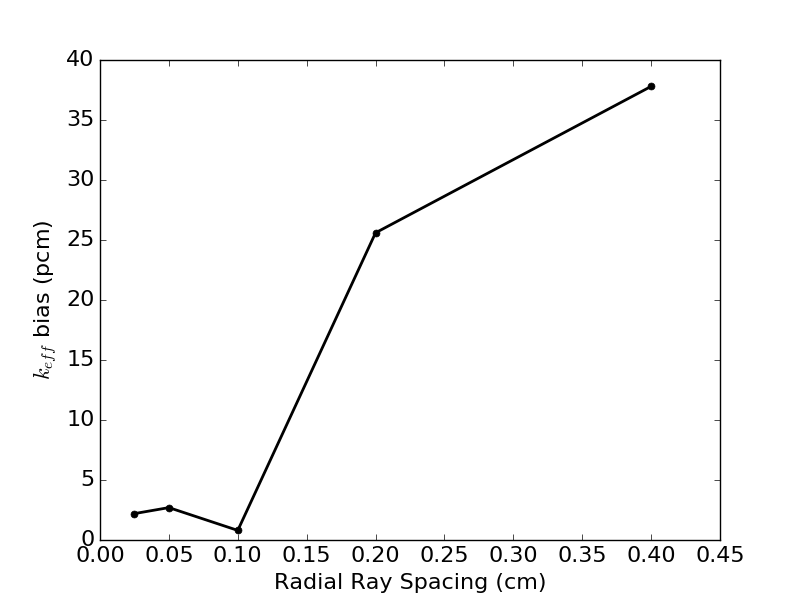
\includegraphics[width=0.7\linewidth]{figures/results/sensitivity/rad_spacing_pcm.png}
	\caption[]{The bias in eigenvalue $k_{\textit{eff}}$ decreasing as radial ray spacing is refined.}
	\label{fig:radial-rs-pcm}
\end{figure}
\begin{figure}[h!]
	\centering
	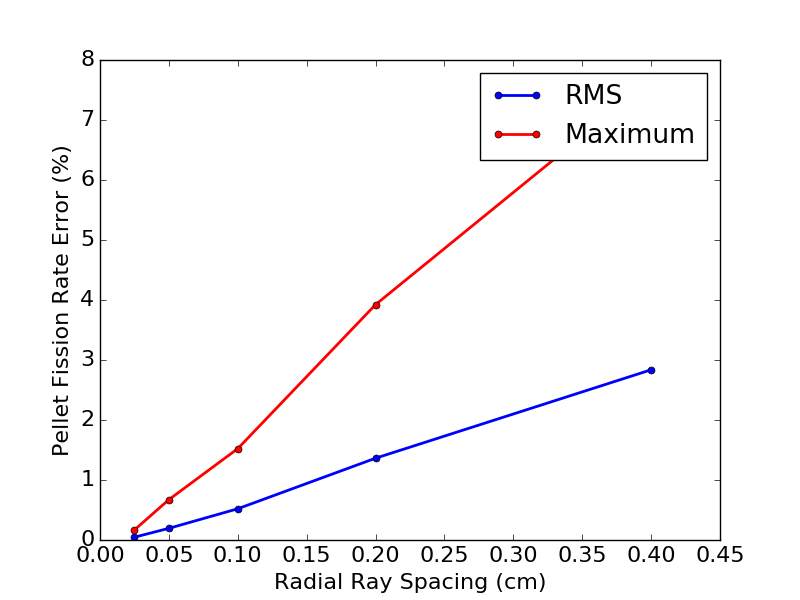
\includegraphics[width=0.7\linewidth]{figures/results/sensitivity/rad_spacing_fr.png}
	\caption[]{The relative pellet-wise fission rate error decreasing as radial ray spacing is refined.}
	\label{fig:radial-rs-fr}
\end{figure}


\subsubsection{Azimuthal Angle Sensitivity}

%FIXME
FIXME: discussion
ref: 256 angles
base: 0.1 cm rad ray spacing


[  NORMAL ]  Azimuthal ray spacing = 0.100000
[  NORMAL ]  Number of polar angles = 10
[  NORMAL ]  Z-spacing = 0.750000


\begin{figure}[h!]
	\centering
	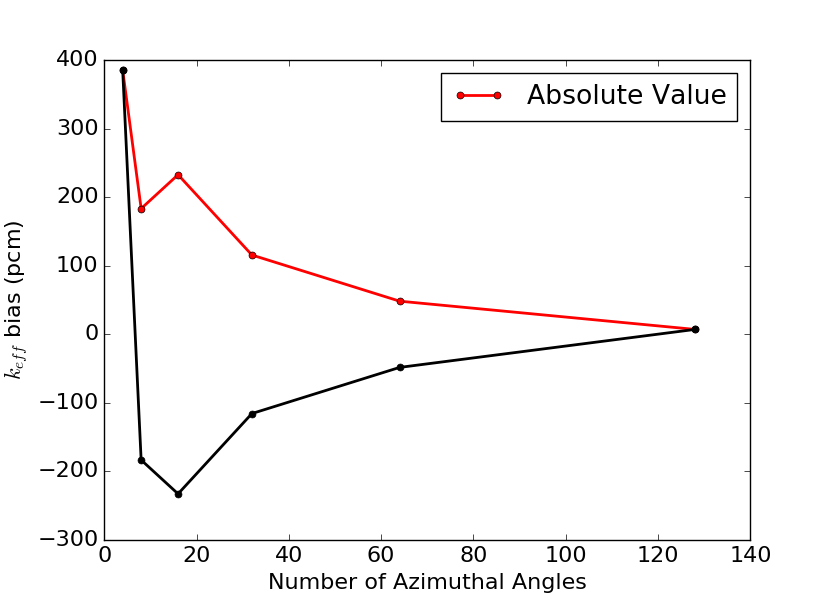
\includegraphics[width=0.7\linewidth]{figures/results/sensitivity/az_angles_pcm.png}
	\caption[]{The bias in eigenvalue $k_{\textit{eff}}$ decreasing as the number of azimuthal angles is increased.}
	\label{fig:az-angles-pcm}
\end{figure}
\begin{figure}[h!]
	\centering
	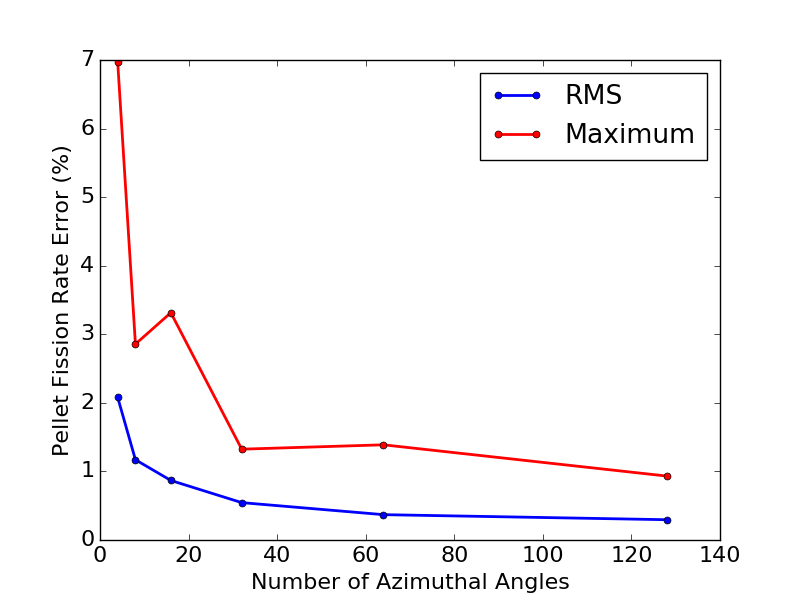
\includegraphics[width=0.7\linewidth]{figures/results/sensitivity/az_angles_fr.png}
	\caption[]{The relative pellet-wise fission rate error decreasing as the number of azimuthal angles is increased.}
	\label{fig:az-angles-fr}
\end{figure}


\section{Axial Sensitivity}
\label{sec:axial-sensitivity}

The previous section studied radial sensitivities, which are known quite well due to extensive experience with 2D \ac{MOC}. Therefore, the studies were a verification that the expected parameters were sufficient to accurately simulate BEAVRS geometries. 

In this section, the axial sensitivities are studied, for which there is much less collective experience. 3D \ac{MOC} solvers have only recently been investigated in great detail. Therefore, rather than verifying a set of \ac{MOC} parameters to be sufficient for accurate simulations, a search is required to find the accurate parameters. This requires some metric for determining whether a simulation is sufficiently accurate.

The following criteria is selected to constitute an accurate simulation: less than 1.0\% RMS pellet fission rate error, less than 3.0\% maximum pellet fission rate error, and less than 20 pcm bias on eigenvalue compared with a converged reference solution. The pellet fission rate is defined to be the fission rate within a given 2.0 cm tall fuel pin region. The reference solution for every case is chosen by further refining the parameter of interest, similar to the radial mesh studies. This allows each parameter to independently be studied.

In this study, the single assembly model detailed in Section~\ref{sec:beavrs-single-assembly} is chosen which contains axial reflectors and grid spacers. It does not contain any inserted rods. Later, a single assembly with inserted rods is analyzed to determine the \ac{MOC} parameters when there are significant axial gradients.

%FIXME
FIXME: discussion

TODO: Talk about axial parameters: angles, spacing, source height.

\subsection{Axial Source Height Sensitivity}

%FIXME
FIXME: discussion
ref: sh = 0.25

base: same as axial ray
ax ray spacing = 1.5/16




\begin{figure}[h!]
	\centering
	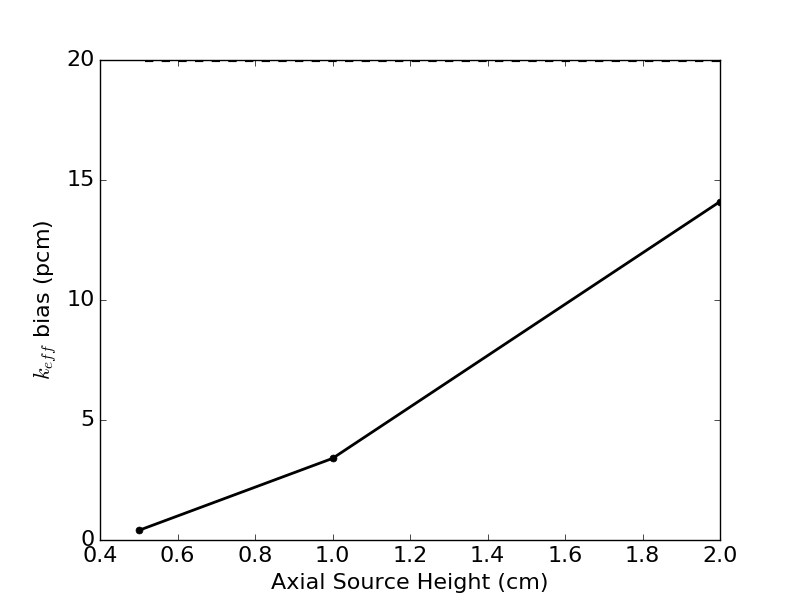
\includegraphics[width=0.7\linewidth]{figures/results/sensitivity/source_height_pcm.png}
	\caption[]{The bias in eigenvalue $k_{\textit{eff}}$ decreasing as axial source height is refined.}
	\label{fig:axial-sh-pcm}
\end{figure}
\begin{figure}[h!]
	\centering
	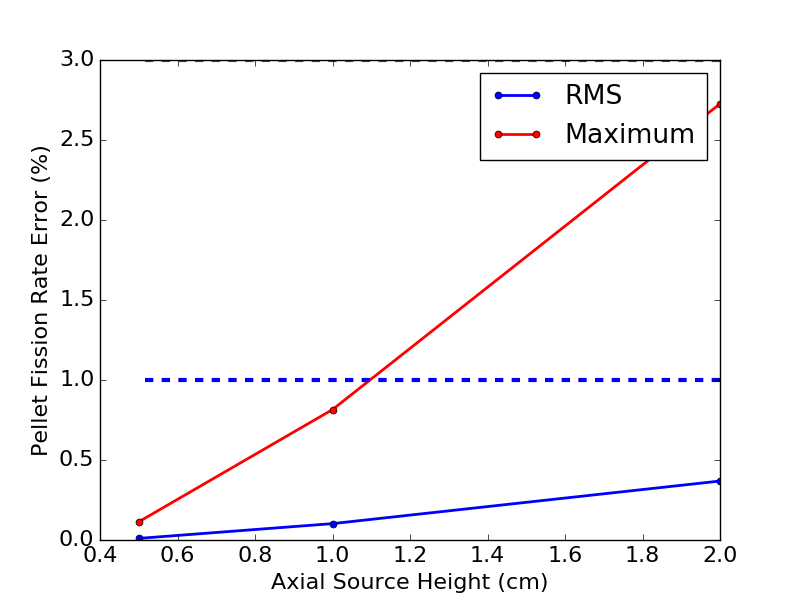
\includegraphics[width=0.7\linewidth]{figures/results/sensitivity/source_height_fr.png}
	\caption[]{The relative pellet-wise fission rate error decreasing as axial source height is refined.}
	\label{fig:axial-sh-fr}
\end{figure}

\subsection{Axial Ray Spacing Sensitivity}

%FIXME
FIXME: discussion
ref: 1.5/32

[  NORMAL ]  Number of azimuthal angles = 32
[  NORMAL ]  Azimuthal ray spacing = 0.100000
[  NORMAL ]  Number of polar angles = 10
source height = 2.0



\begin{figure}[h!]
	\centering
	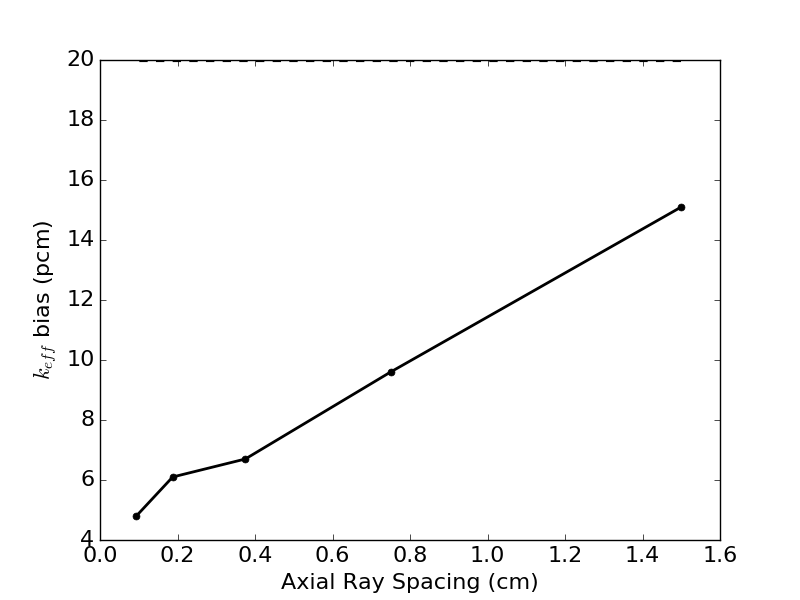
\includegraphics[width=0.7\linewidth]{figures/results/sensitivity/z_spacing_pcm.png}
	\caption[]{The bias in eigenvalue $k_{\textit{eff}}$ decreasing as axial ray spacing is refined.}
	\label{fig:axial-rs-pcm}
\end{figure}
\begin{figure}[h!]
	\centering
	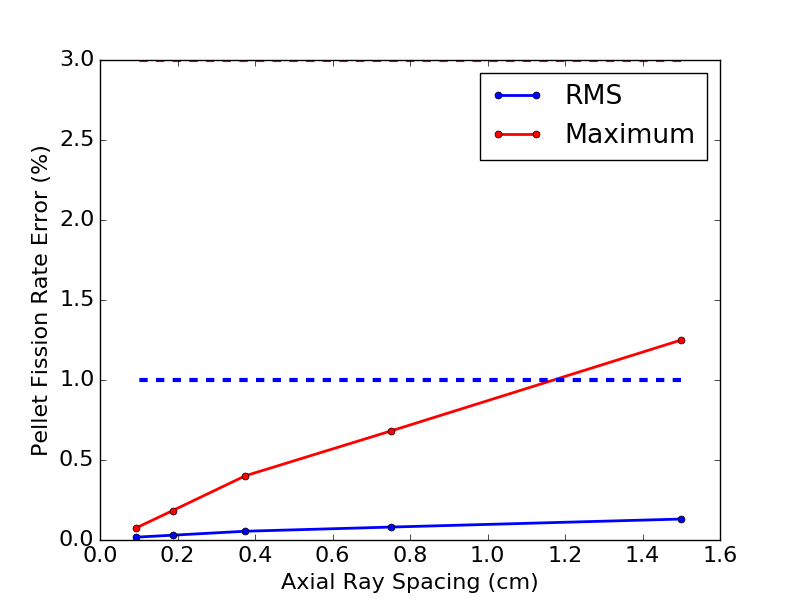
\includegraphics[width=0.7\linewidth]{figures/results/sensitivity/z_spacing_fr.png}
	\caption[]{The relative pellet-wise fission rate error decreasing as axial ray spacing is refined.}
	\label{fig:axial-rs-fr}
\end{figure}

\subsection{Polar Angle Sensitivity}

%FIXME
FIXME: discussion
ref: 32

[  NORMAL ]  Number of azimuthal angles = 32
[  NORMAL ]  Azimuthal ray spacing = 0.100000
[  NORMAL ]  Z-spacing = 0.250000

\begin{figure}[h!]
	\centering
	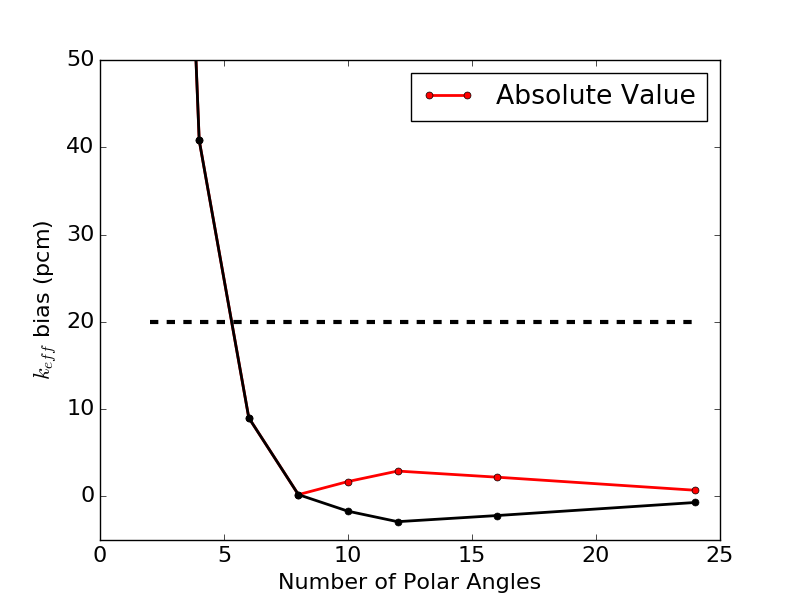
\includegraphics[width=0.7\linewidth]{figures/results/sensitivity/polar_angles_pcm.png}
	\caption[]{The bias in eigenvalue $k_{\textit{eff}}$ decreasing as the number of polar angles is increased.}
	\label{fig:polar-angles-pcm}
\end{figure}
\begin{figure}[h!]
	\centering
	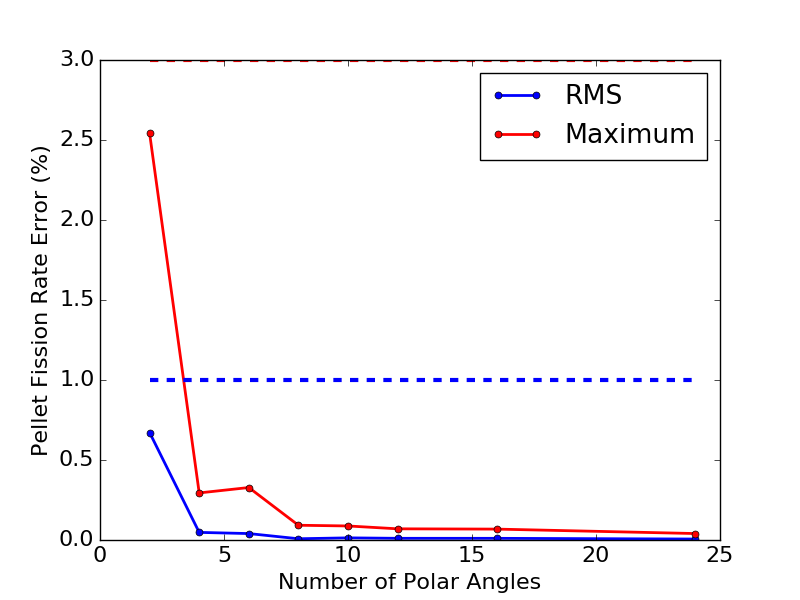
\includegraphics[width=0.7\linewidth]{figures/results/sensitivity/polar_angles_fr.png}
	\caption[]{The relative pellet-wise fission rate error decreasing as the number of polar angles is increased.}
	\label{fig:polar-angles-fr}
\end{figure}


\section{Axial Sensitivity on a Rodded Assembly}
\label{sec:axial-sensitivity-rodded}

\subsection{Axial Source Height Sensitivity}

%FIXME
FIXME: discussion
base: 1.5 / 16
ref: 0.25

\begin{figure}[h!]
	\centering
	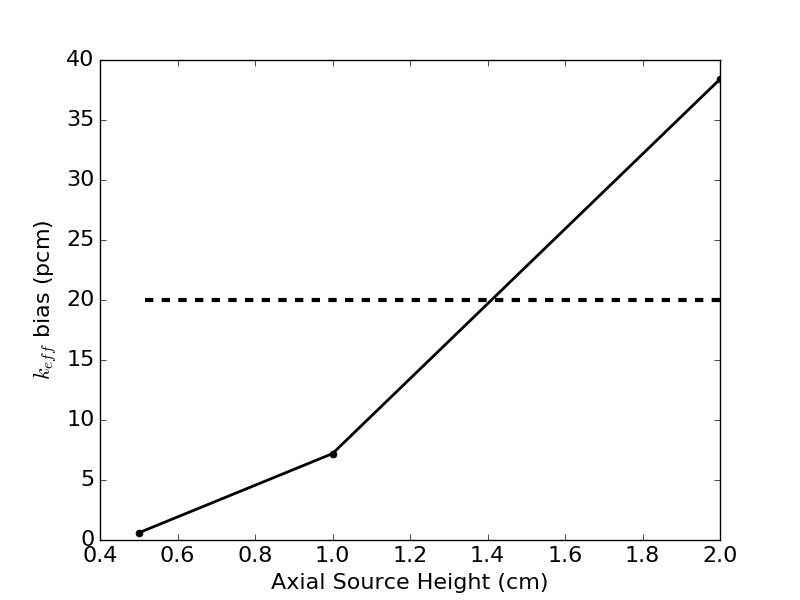
\includegraphics[width=0.7\linewidth]{figures/results/sensitivity/rodded_source_height_pcm.png}
	\caption[]{The bias in eigenvalue $k_{\textit{eff}}$ decreasing as axial source height is refined.}
	\label{fig:rodded-axial-sh-pcm}
\end{figure}
\begin{figure}[h!]
	\centering
	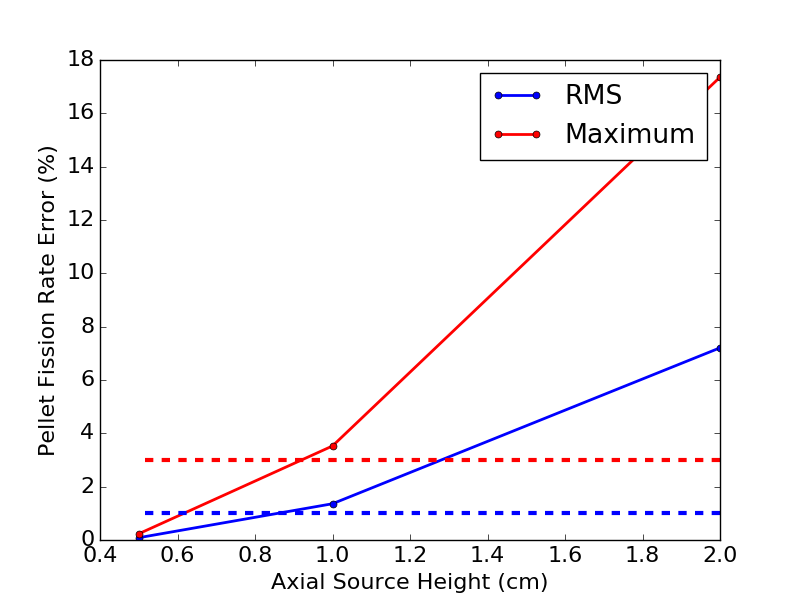
\includegraphics[width=0.7\linewidth]{figures/results/sensitivity/rodded_source_height_fr.png}
	\caption[]{The relative pellet-wise fission rate error decreasing as axial source height is refined.}
	\label{fig:rodded-axial-sh-fr}
\end{figure}

\subsection{Axial Ray Spacing Sensitivity}

%FIXME
FIXME: discussion
ref: 1.5/64
base: 0.5 source height

\begin{figure}[h!]
	\centering
	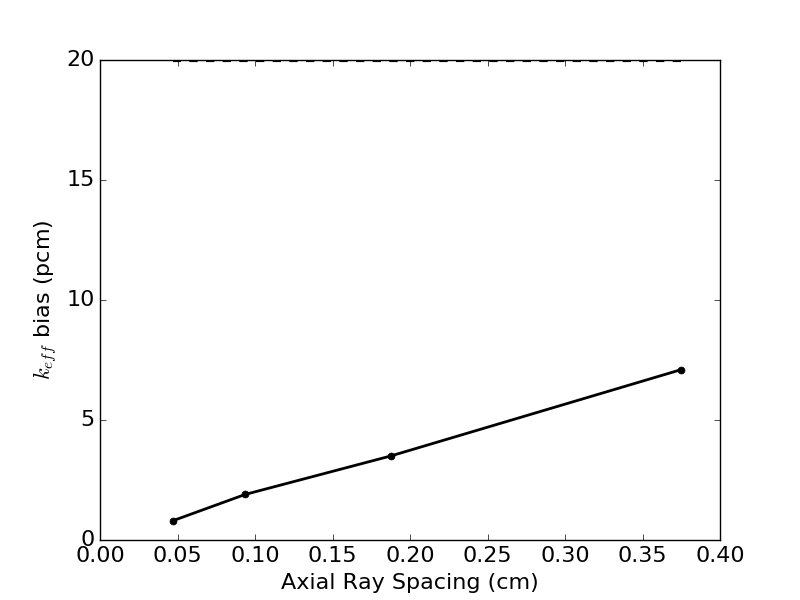
\includegraphics[width=0.7\linewidth]{figures/results/sensitivity/rodded_z_spacing_pcm.png}
	\caption[]{The bias in eigenvalue $k_{\textit{eff}}$ decreasing as axial ray spacing is refined.}
	\label{fig:rodded-axial-rs-pcm}
\end{figure}
\begin{figure}[h!]
	\centering
	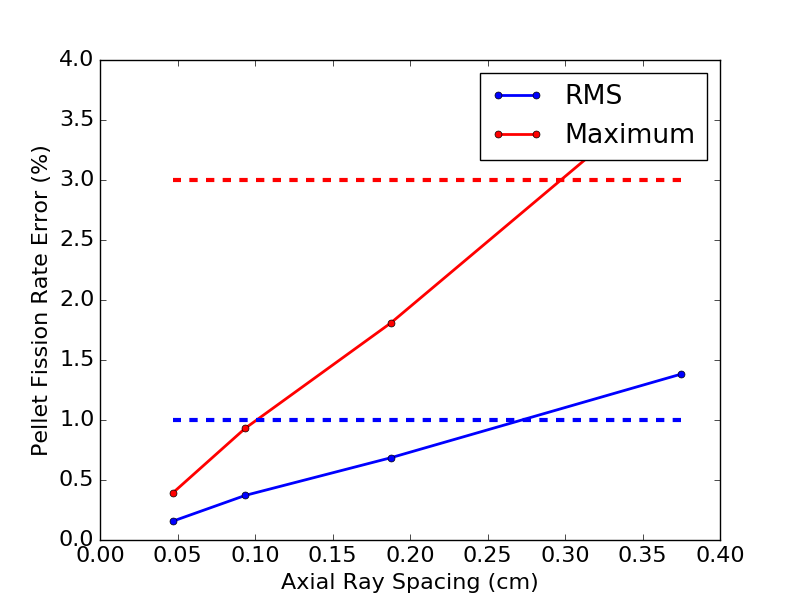
\includegraphics[width=0.7\linewidth]{figures/results/sensitivity/rodded_z_spacing_fr.png}
	\caption[]{The relative pellet-wise fission rate error decreasing as axial ray spacing is refined.}
	\label{fig:rodded-axial-rs-fr}
\end{figure}

\subsection{Polar Angle Sensitivity}

%FIXME
FIXME: discussion

SAME as unrodded

\begin{figure}[h!]
	\centering
	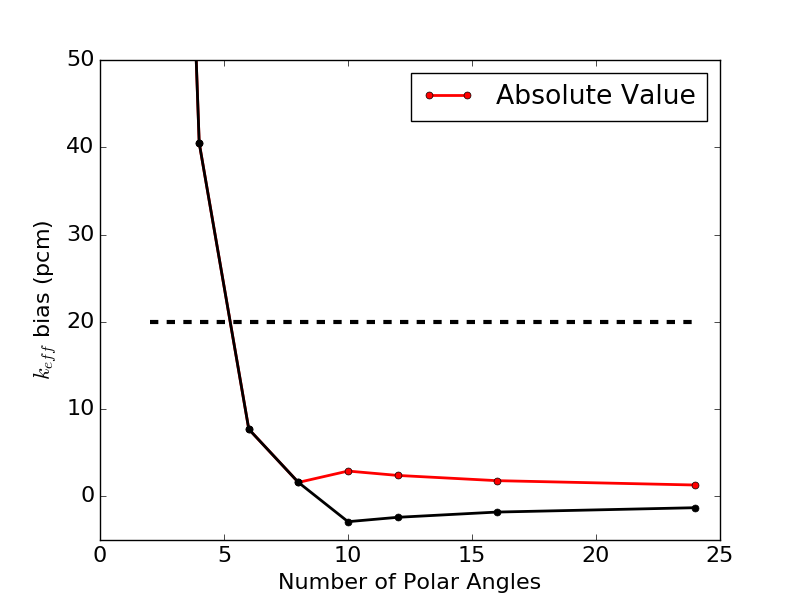
\includegraphics[width=0.7\linewidth]{figures/results/sensitivity/rodded_polar_angles_pcm.png}
	\caption[]{The bias in eigenvalue $k_{\textit{eff}}$ decreasing as the number of polar angles is increased.}
	\label{fig:rodded-polar-angles-pcm}
\end{figure}
\begin{figure}[h!]
	\centering
	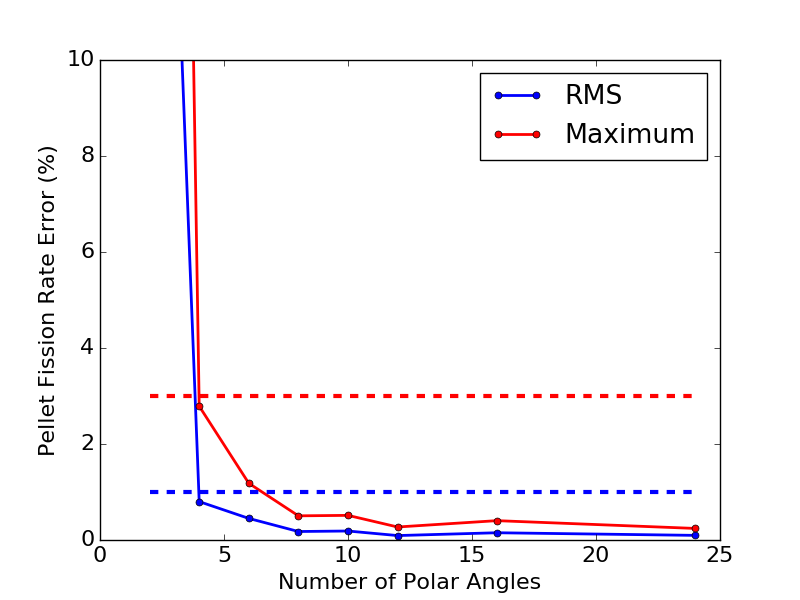
\includegraphics[width=0.7\linewidth]{figures/results/sensitivity/rodded_polar_angles_fr.png}
	\caption[]{The relative pellet-wise fission rate error decreasing as the number of polar angles is increased.}
	\label{fig:rodded-polar-angles-fr}
\end{figure}

\section{Comparison with Flat Source MOC}
\label{sec:flat-linear-comparision}


\section{Conclusion}
\label{sec:sensitivity-conclusion}

Create table of parameters required to converge PWR problems with 3D MOC

\clearpage

\vfill
\begin{highlightsbox}[frametitle=Highlights]
\begin{itemize}
  \item A framework consisting of OpenMC, OpenMOC and OpenCG was used to explore \ac{MC}-based \ac{MGXS} generation methods for fine-mesh transport calculations.
  \item A fully-featured Python \ac{API} was developed to support input generation and downstream processing of large tally datasets for OpenMC.
  \item The \texttt{openmc.mgxs} Python module was created to generate \ac{MGXS} from OpenMC tallies. The distributed cell tally algorithm was implemented to generate pin-wise \ac{MGXS} in large, heterogeneous geometries.
  \item New features were added to the deterministic multi-group OpenMOC code to enable it to use \ac{MGXS} generated by \texttt{openmc.mgxs} in 2D \ac{MOC} calculations.
  \item The OpenCG code was created to facilitate data processing and transfer on the combinatorial geometry meshes used by OpenMC and OpenMOC.
  \item OpenCG's \ac{LNS} and region differentiation algorithms were crucial components for the spatial homogenization methodologies developed in Chaps.~\Crefrange{chap:benchmarks}{chap:results}.  
\end{itemize}
\end{highlightsbox}
\vfill